\section{Introduction}
\label{sec:intro}
Learned embeddings support retrieval-augmented generation~\cite{lewis2020rag}, recommendation and search~\cite{sobot2023voyager}, code assistance~\cite{fu2025copilot}, multimodal retrieval~\cite{google2026embedding}, and protein-structure search over 214 million predicted structures~\cite{segura2026structure}. Across these applications, embeddings become reusable data objects stored and accessed through vector-similarity queries.

Serving these collections couples three system costs: construction time, memory, and query throughput. A million 1,536-dimensional FP32 vectors occupy approximately 5.72 GiB before graph edges, identifiers, or query workspaces are stored. A graph search repeatedly fetches small, irregular subsets of this representation, while graph construction performs many more comparisons to discover and prune candidate edges. Reducing the representation involved in those comparisons can therefore improve both index preparation and recurring search cost.

Compressed graph indices already exploit this opportunity. Locally adaptive vector quantization (LVQ) supports graph construction and search with compact scalar codes~\cite{aguerrebere2023lvq}. NGT-QG and SymphonyQG arrange quantized neighborhoods for batched SIMD scoring~\cite{ngt,gou2025symphony}, and Lucene's Better Binary Quantization (BBQ) combines very small database codes with higher-precision query codes~\cite{trent2024bbq,veasey2024osq}. The relevant design space thus includes the graph, its scoring function, and the memory layout.

Aggressive compression introduces a particular tension within that design space. A cheaper score is useful only if it saves more work than its errors create. Approximate scores determine which vertices are expanded, which candidates survive a bounded beam, and which survivors receive expensive exact evaluation. These decisions determine the neighbors available to final reranking. Thus, the cost of low-bit search depends on both \emph{the price of each comparison} and \emph{the number and quality of the comparisons induced by the representation}.

Our insight is that construction and navigation can share two coordinate bits while using different scoring rules. Construction discovers candidates with two-plane Hamming scores and orders the candidate pool with an integer proxy. Query navigation combines these bits with per-vector reconstruction amplitudes and norms to order the frontier and candidate pool. Original vectors are accessed only for bounded final reranking. This division of precision reduces repeated construction work and navigation storage while preserving the candidates needed for accurate retrieval on semantic embeddings.

The distinction between visiting and retaining candidates is central. On a controlled Cohere-200K experiment, an unnormalized reconstruction inner product visits a set covering 96.31\% of the true top ten, but retains only 76.93\% in its final beam at width 64. Reconstruction L2 reaches 96.48\% Recall@10. This is a failure of approximate selection inside the search, even though the graph has exposed many correct neighbors. It motivates using the same norm-aware score for both expansion and candidate retention.

We implement this design as \quiver{} in TriviumDB. Parallel insertion and deferred reverse-edge pruning accelerate construction; packed bit planes, population-count kernels, shared adjacency, and reusable thread-local state accelerate queries (Figure~\ref{fig:pipeline}). The resulting index occupies a measured Pareto-frontier position on all three core workloads when achieved recall, throughput, preparation time, and memory are considered jointly, whether or not memory includes the original vectors. On Cohere-5M, it retains 97\% of SymphonyQG's 32-thread throughput with 54\% less preparation time and 47\% less total logical memory. An SSD mode keeps this navigation path in memory and reads INT8-quantized vectors for bounded reranking, serving Cohere-5M at about 5 GiB of steady-state process RSS.

We make three contributions:
\begin{itemize}
    \item A two-bit graph-index design that assigns inexpensive integer scoring to construction, reconstruction-aware scoring to navigation and retention, and bounded original-vector access to final ranking.
    \item An implementation that makes this precision split effective through parallel construction, deferred pruning, bitwise scoring, shared adjacency storage, and reusable query state, with separately measured preparation and memory costs, and an SSD mode that fetches INT8-quantized reranking rows in one bounded batch per query.
    \item Evidence of Pareto-efficient indexing on three core workloads, supported by comparisons with 30 external modes, a 21-dataset applicability study, held-out queries, and controlled experiments separating construction, navigation, candidate retention, and reranking.
\end{itemize}

\begin{figure*}[!t]
\centering
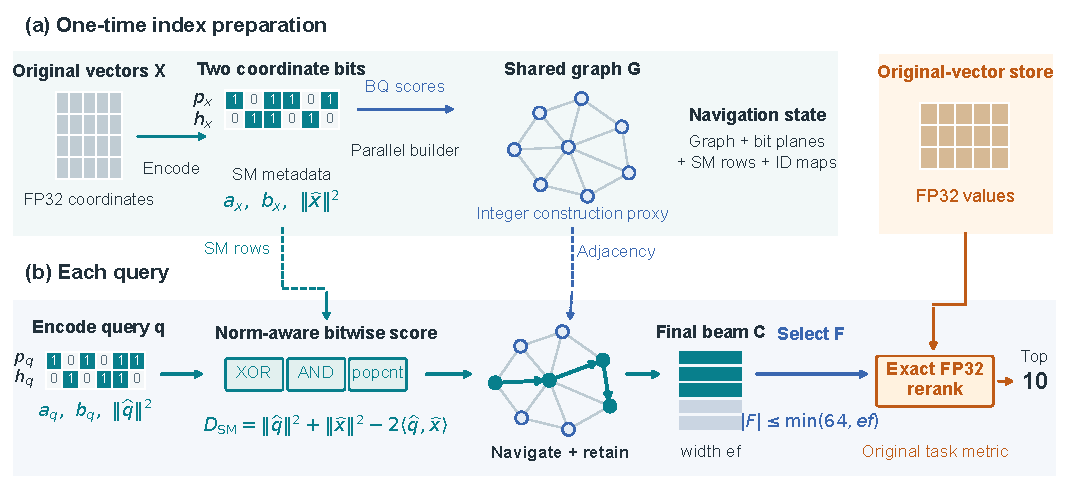
\includegraphics[width=\textwidth]{pipeline.pdf}
\caption{Precision across the QuIVer lifecycle. (a) Two coordinate bits support integer BQ construction; per-vector metadata prepares SM-L2 navigation. (b) Bitwise scoring drives traversal and retention; at most $\min(64,ef)$ candidates receive FP32 reranking. Dashed links supply persistent navigation state, and amber supplies original values. Bit patterns and graph layouts are schematic.}
\label{fig:pipeline}
\end{figure*}
